\documentclass[11pt,a4paper]{article}

\usepackage[T1]{fontenc}
\usepackage[utf8]{inputenc}
\usepackage[margin=1in]{geometry}
\usepackage{amsmath,amssymb}
\usepackage{booktabs}
\usepackage{array}
\usepackage{graphicx}
\usepackage{xcolor}
\usepackage{microtype}
\usepackage{enumitem}
\usepackage{caption}
\usepackage{subcaption}
\usepackage[hidelinks]{hyperref}

\definecolor{accent}{HTML}{1a5276}
\definecolor{lightgray}{HTML}{f2f3f4}

\captionsetup{font=small,labelfont=bf}

\newcommand{\cmark}{\textcolor{green!50!black}{kept}}
\newcommand{\xmark}{\textcolor{red!60!black}{dropped}}

\title{\textbf{Packaging Material Difference Mining}\\[2mm]
\large CyberAI Cup 2026 --- Task 1 --- Full Technical Report}
\author{}
\date{Written 2026-08-21}

\begin{document}

\maketitle
\vspace{-4em}

\begin{center}
\fcolorbox{accent}{lightgray}{%
\begin{minipage}{0.94\textwidth}
\centering
\textbf{Result: pooled 5-fold out-of-fold global F1 = 0.9465}\\
(0.9435 after removing threshold-selection bias)\\[1mm]
\small Starting point 0.9049 (single fold). The 0.97 target was \emph{not} reached; \S 8 shows it
was not reachable with this candidate set --- a perfect rescorer caps out at 0.9801.
\end{minipage}}
\end{center}

\section{The task and the metric}

Given a pair of images --- a clean design \emph{template} and a \emph{photograph} of the printed
packaging --- predict bounding boxes around every genuine \emph{content} difference (text,
graphics, layout). Printing and scanning artefacts are \emph{not} differences.

Scoring is \textbf{global F1}: true positives, false positives and false negatives accumulate
across \emph{every} image \emph{before} precision and recall are computed. A per-image average
would let one catastrophic image hide among 99 good ones; global F1 does not. Fifty false
positives on one page damage the score exactly as much as fifty spread across fifty pages. A
prediction is a true positive when its IoU with an unmatched ground-truth box is $\geq 0.5$.

\textbf{Data:} 200 annotated training pairs (1{,}407 boxes), 100 unlabelled test pairs, 2.5\,GB.

\section{What the data actually looks like}

Every figure below is reproducible with \texttt{scripts/analyze\_dataset.py}. These measurements,
not intuition, drove the architecture.

\begin{table}[h!]
\centering
\small
\renewcommand{\arraystretch}{1.25}
\begin{tabular}{@{}p{3.4cm}p{5.4cm}p{6.2cm}@{}}
\toprule
\textbf{Property} & \textbf{Measurement} & \textbf{Consequence} \\
\midrule
Annotation density & 1{,}407 boxes / 200 pairs, 3--11 per image, median 7 & expect $\sim$7 predictions per test image \\
Image geometry & template and photo identical size (all 200 pairs) & full-resolution tiling, no resizing \\
Alignment & phase-correlation residual p95 $\leq$ 0.26\,px & registration is \emph{not} the problem \\
Box size & median 22$\times$22\,px; 419/1407 both sides $<$16\,px; 83 exactly 8$\times$8 & \textbf{output stride 2, not 4} \\
Change polarity & 842 additions, 558 modifications, \textbf{0 deletions} & licenses the polarity filter \\
Degradation & photo blurred/noisy/tone-shifted; $\sim$18\% heavy shadow & blur-matching + ink maps \\
\bottomrule
\end{tabular}
\end{table}

\textbf{The two hard parts, quantified.}

\begin{enumerate}[leftmargin=1.6em]
\item \emph{Precision.} A naive normalized-difference baseline reaches recall 0.57 at precision
\textbf{0.015} --- global F1 \textbf{0.0293}. Every glyph edge fires because the photo is softer
than the template. Blur-matching the template before differencing is what makes the problem
tractable at all.
\item \emph{Localization.} An 8$\times$8 box at IoU 0.5 tolerates roughly 2.7\,px of error.
Thresholded difference blobs match ground truth at median IoU 0.58, with only 34\% correct within
$\pm$2\,px on all sides. Hence sub-pixel box regression rather than blob thresholding.
\end{enumerate}

\section{Architecture}

\begin{figure}[h!]
\centering
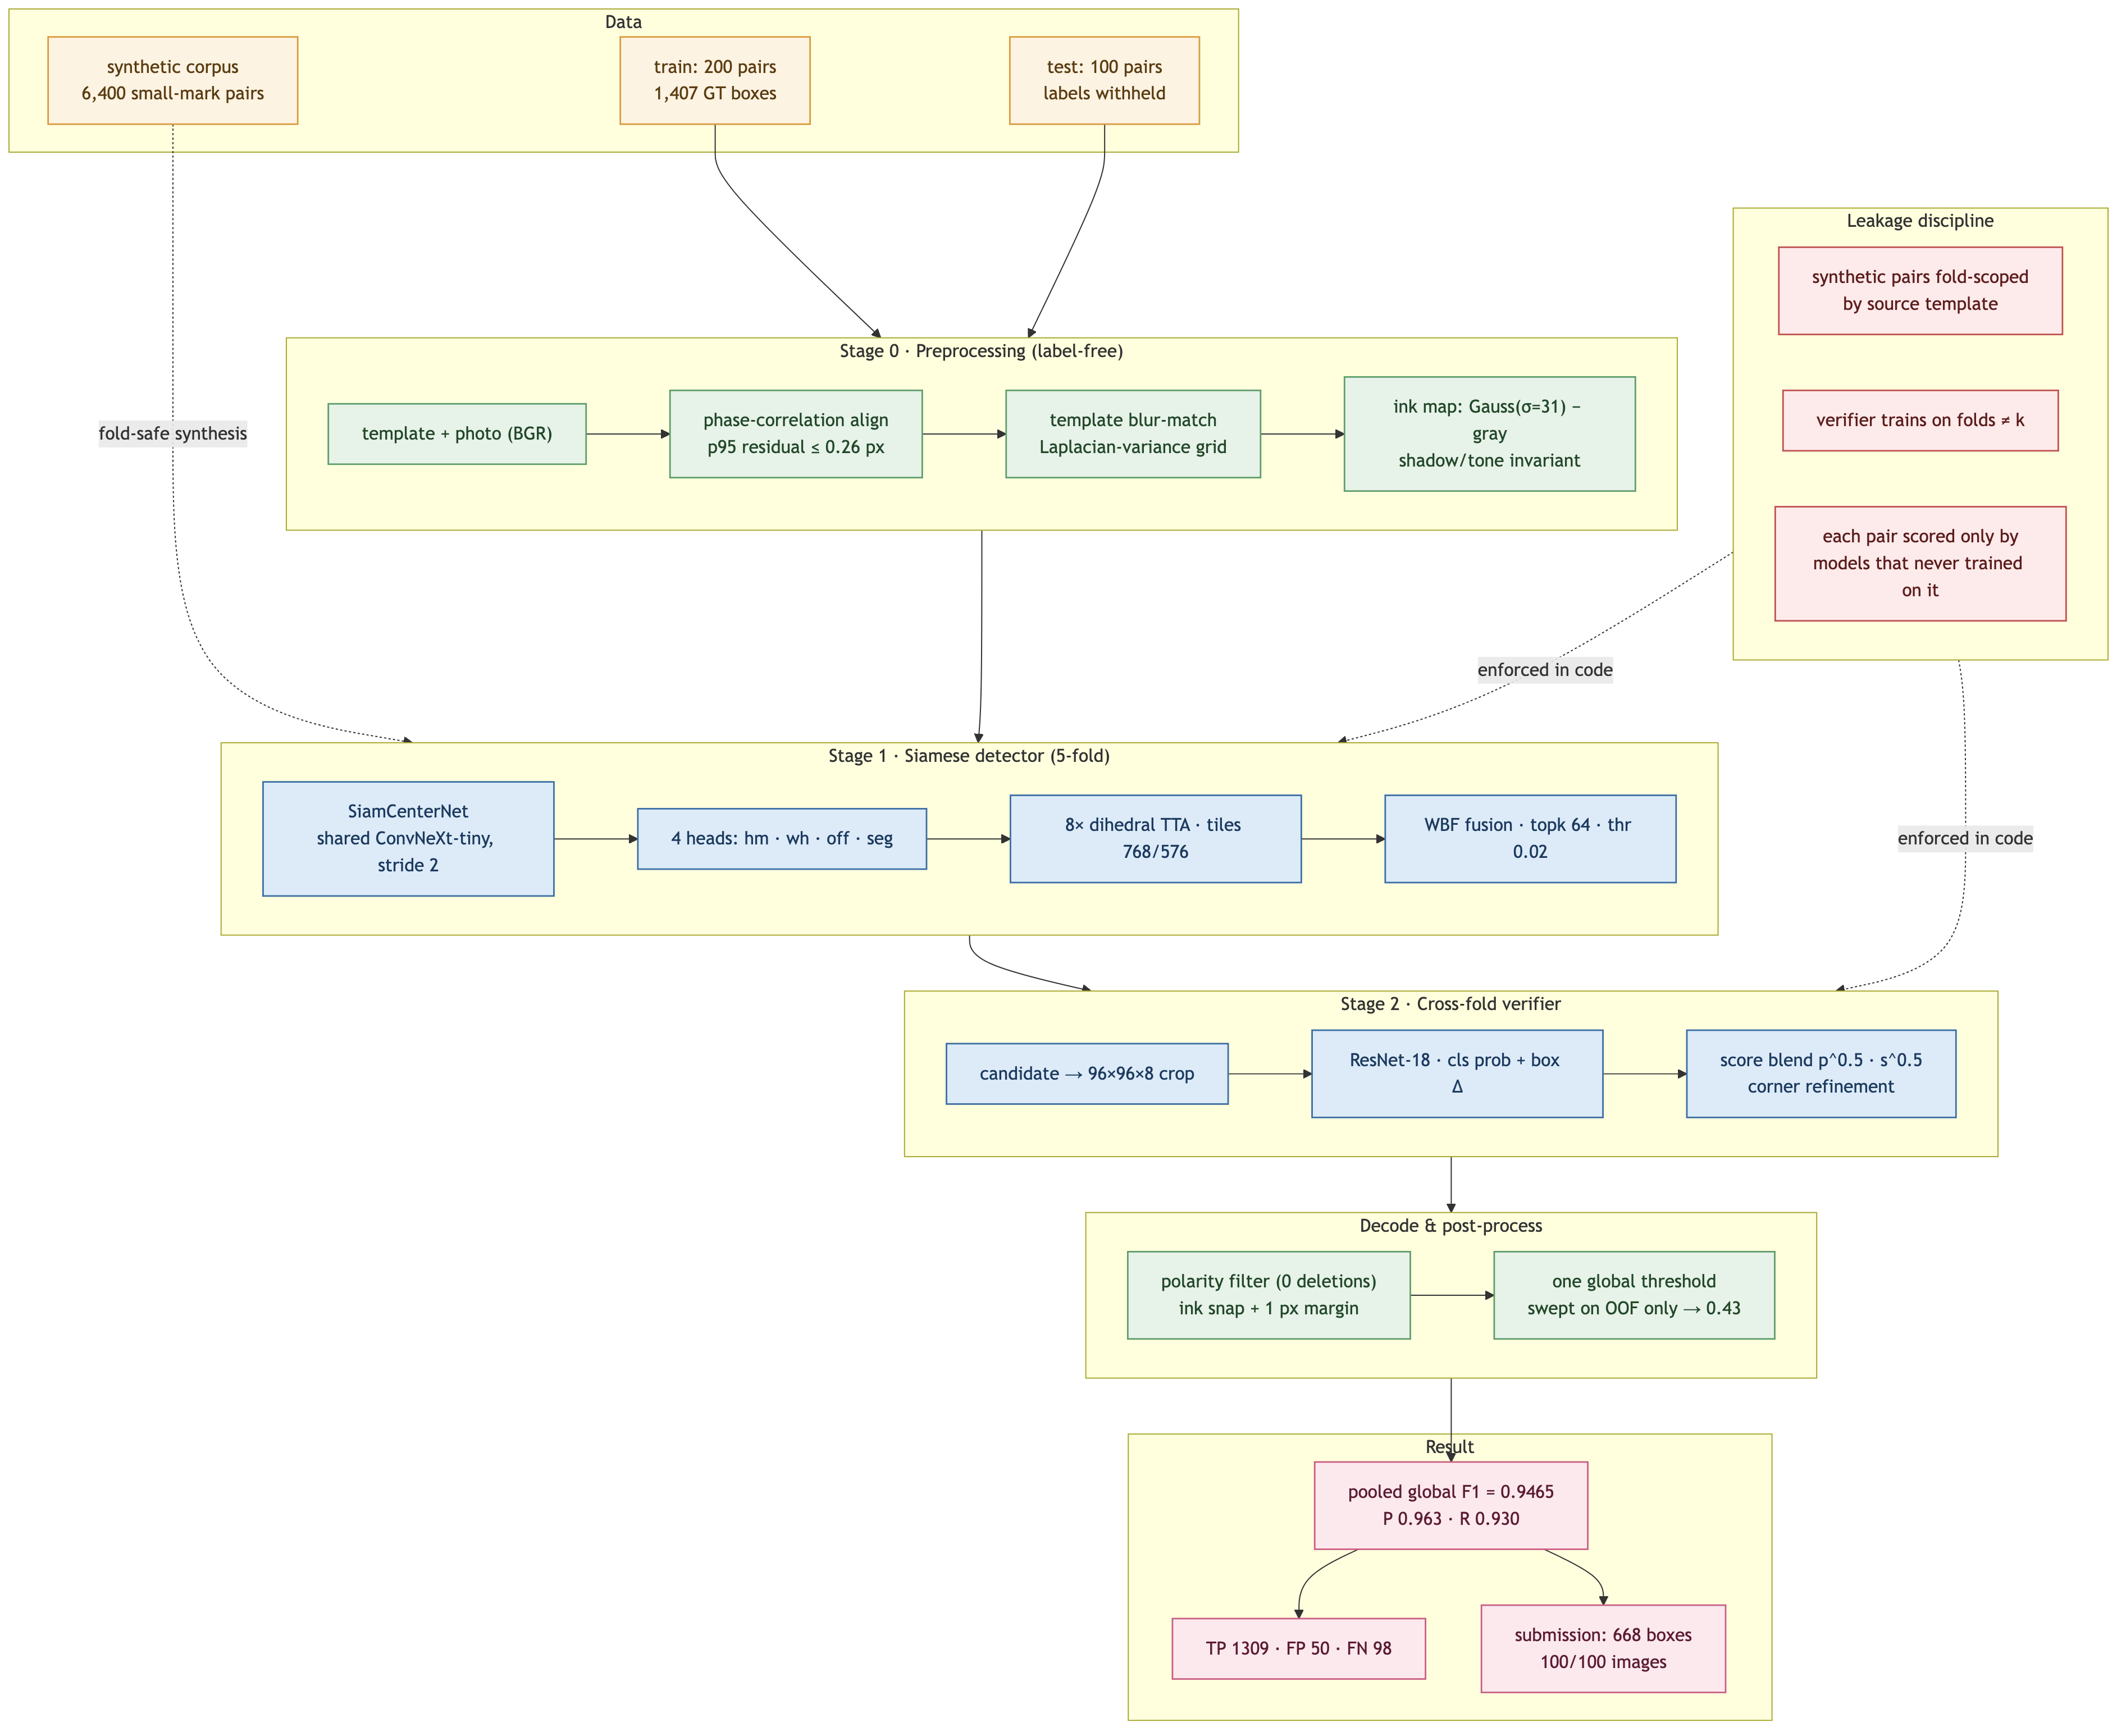
\includegraphics[width=\textwidth]{../report/diagrams/task1_pipeline.png}
\caption{End-to-end Task 1 pipeline: preprocessing, siamese CenterNet detector, patch verifier,
and decoding into the final submission.}
\label{fig:pipeline}
\end{figure}

\subsection{Stage 0 --- preprocessing (\texttt{src/pmdm/preprocess.py})}

Verify alignment by phase correlation and translate if needed. Blur-match the template to the
photo by searching a $\sigma$ grid for the blur that equalizes Laplacian variance. Compute an
``ink map'' per image, $\mathrm{GaussianBlur}(\mathrm{gray},\,\sigma{=}31) - \mathrm{gray}$,
which is invariant to shadow and tone shift. Cache four PNGs per pair. \emph{Label-free
throughout.}

\subsection{Stage 1 --- siamese CenterNet (\texttt{src/pmdm/model.py})}

A shared-weight ConvNeXt-tiny encoder runs over two 4-channel streams (BGR $+$ ink map). Features
fuse at every scale as $\mathrm{conv}\bigl(\mathrm{concat}(a,\,b,\,|a-b|)\bigr)$ --- the U-Net
SiamDiff/SiamConc shape --- and decode through a U-Net path to \textbf{output stride 2}, with a
stride-2 stem taken straight from the stacked input so fine detail is not invented by upsampling.

Stride 2 is load-bearing: 83 ground-truth boxes are 8$\times$8\,px and would occupy a 2$\times$2
cell at the stride 4 a standard CenterNet uses.

Four heads: Gaussian-focal centre heatmap, width/height, sub-pixel offset, and an auxiliary change
mask. Trained on 768\,px tiles, 60\% of them sampled around an annotated difference.

\begin{figure}[h!]
\centering
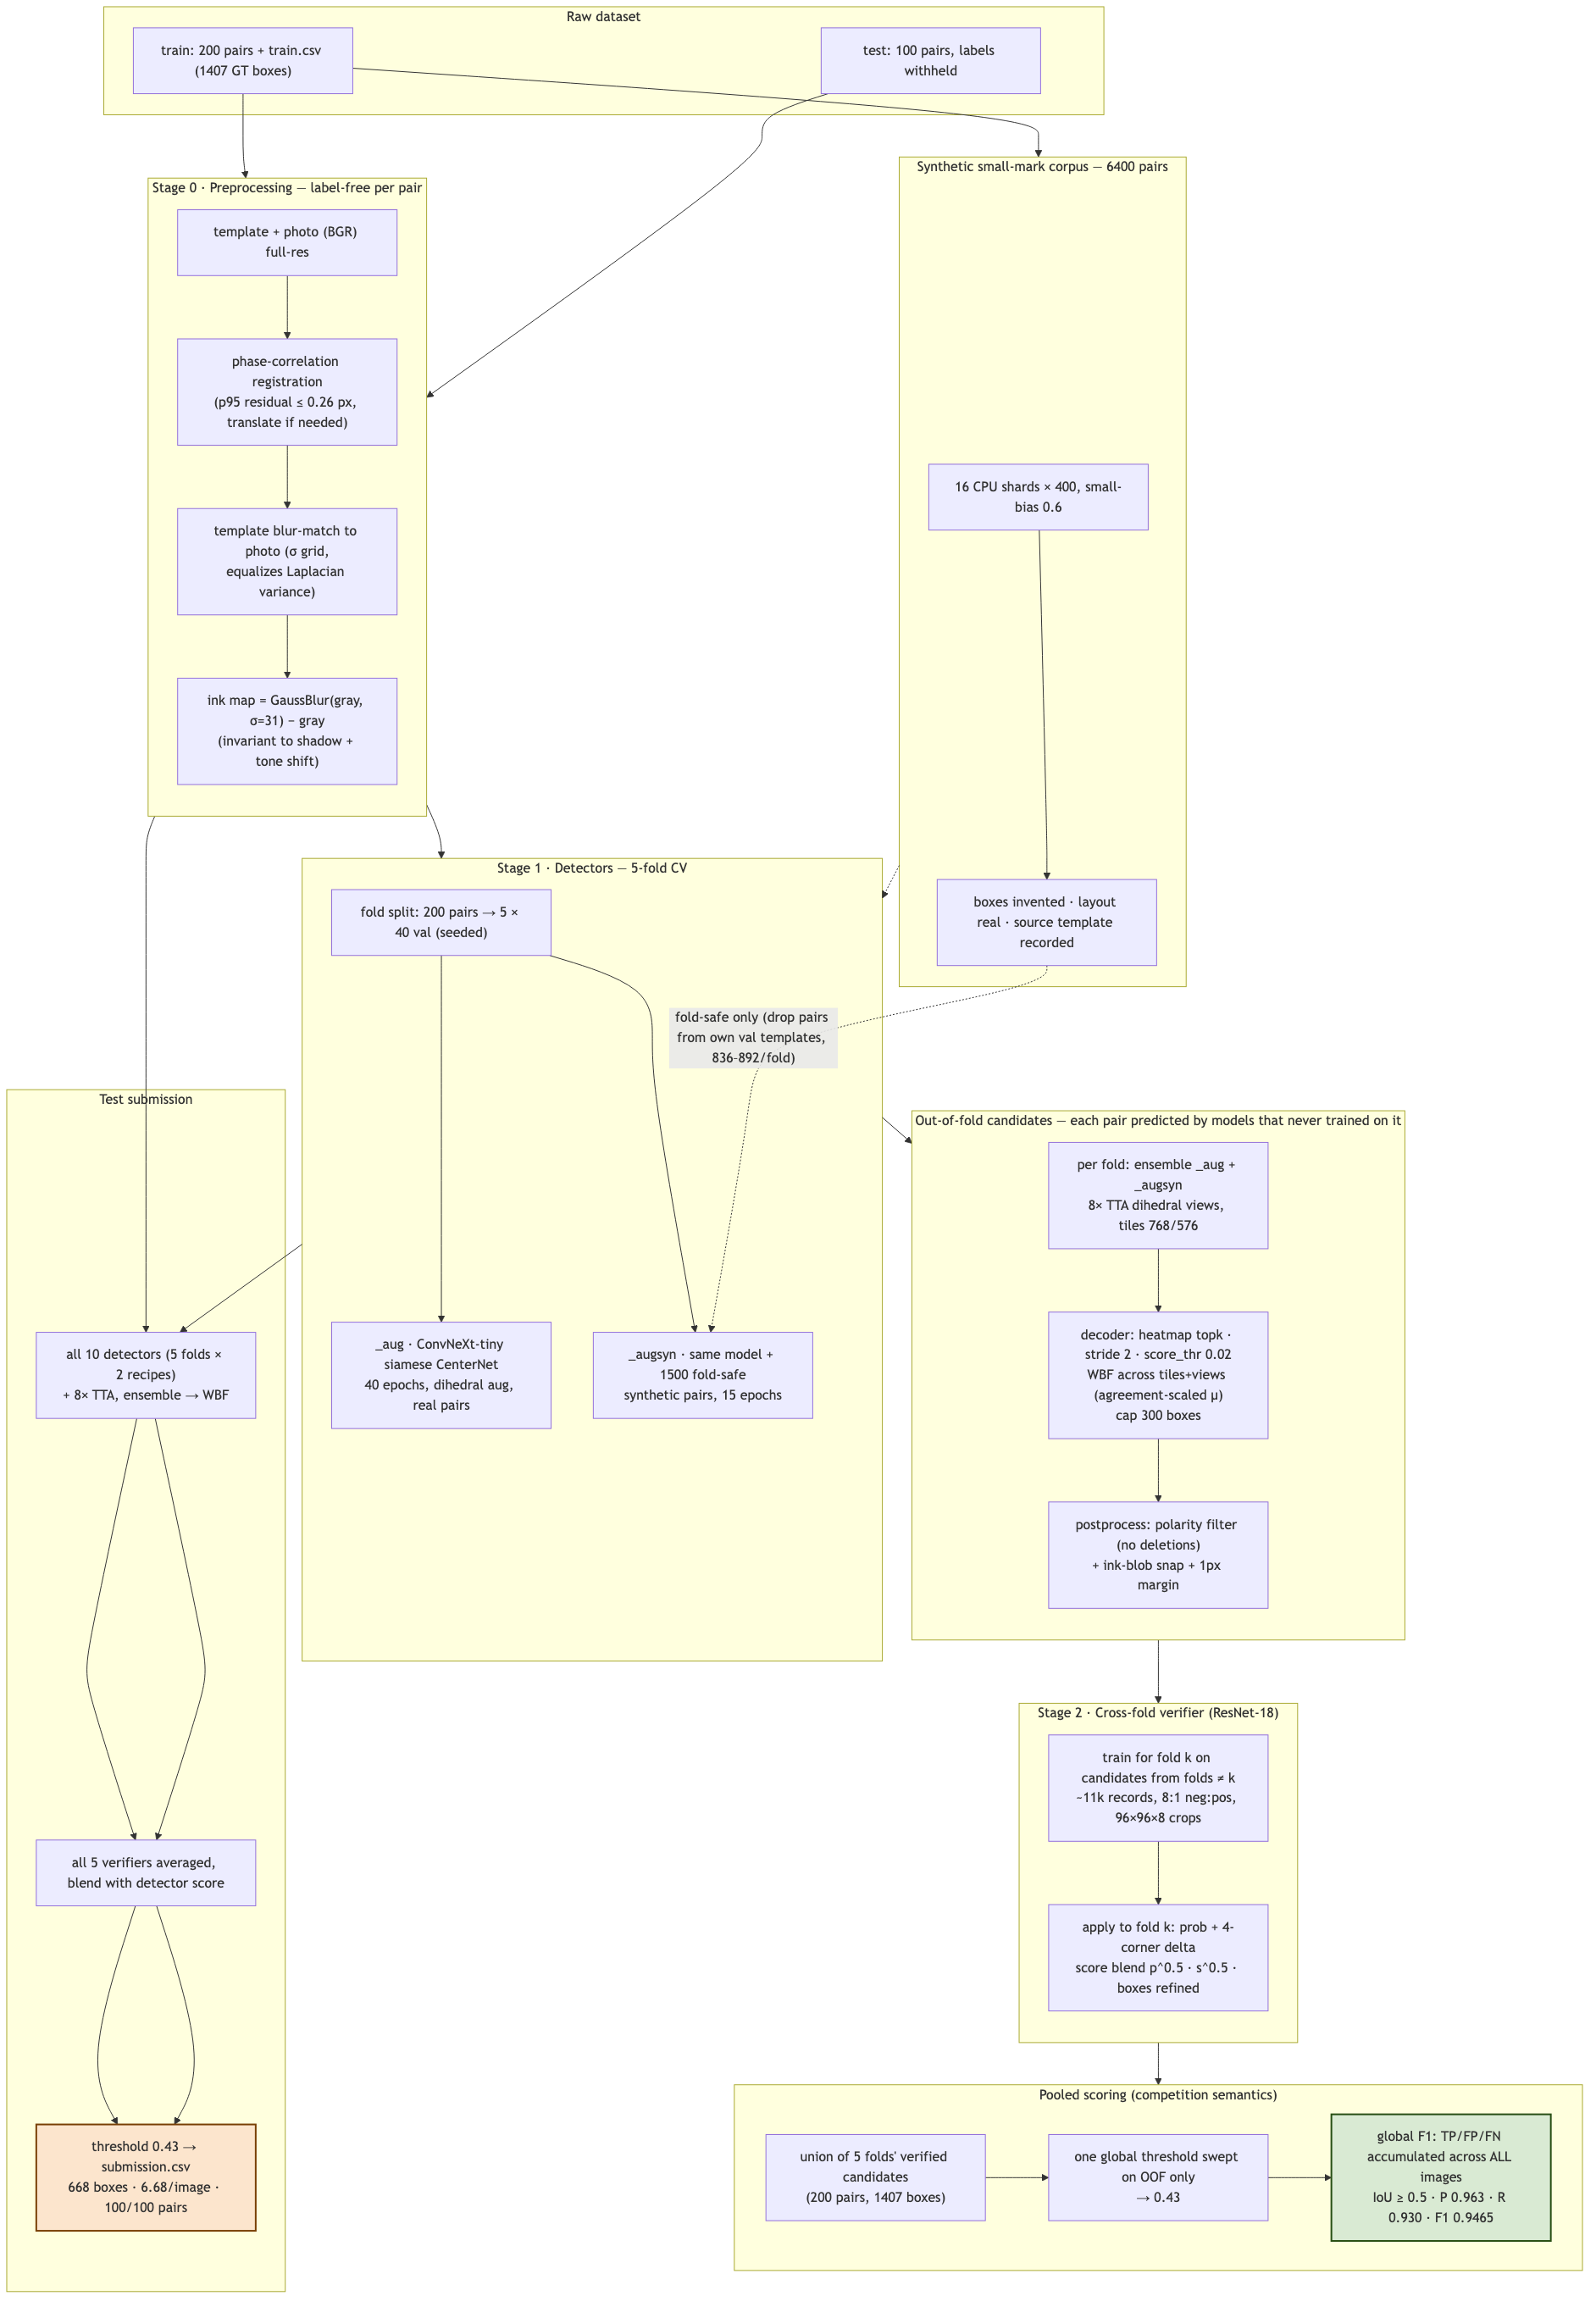
\includegraphics[width=0.72\textwidth]{../diagrams/architecture_pipeline.png}
\caption{Architecture detail: siamese encoder streams, per-scale fusion, and stride-2 U-Net
decoder heads.}
\label{fig:arch}
\end{figure}

\begin{figure}[h!]
\centering
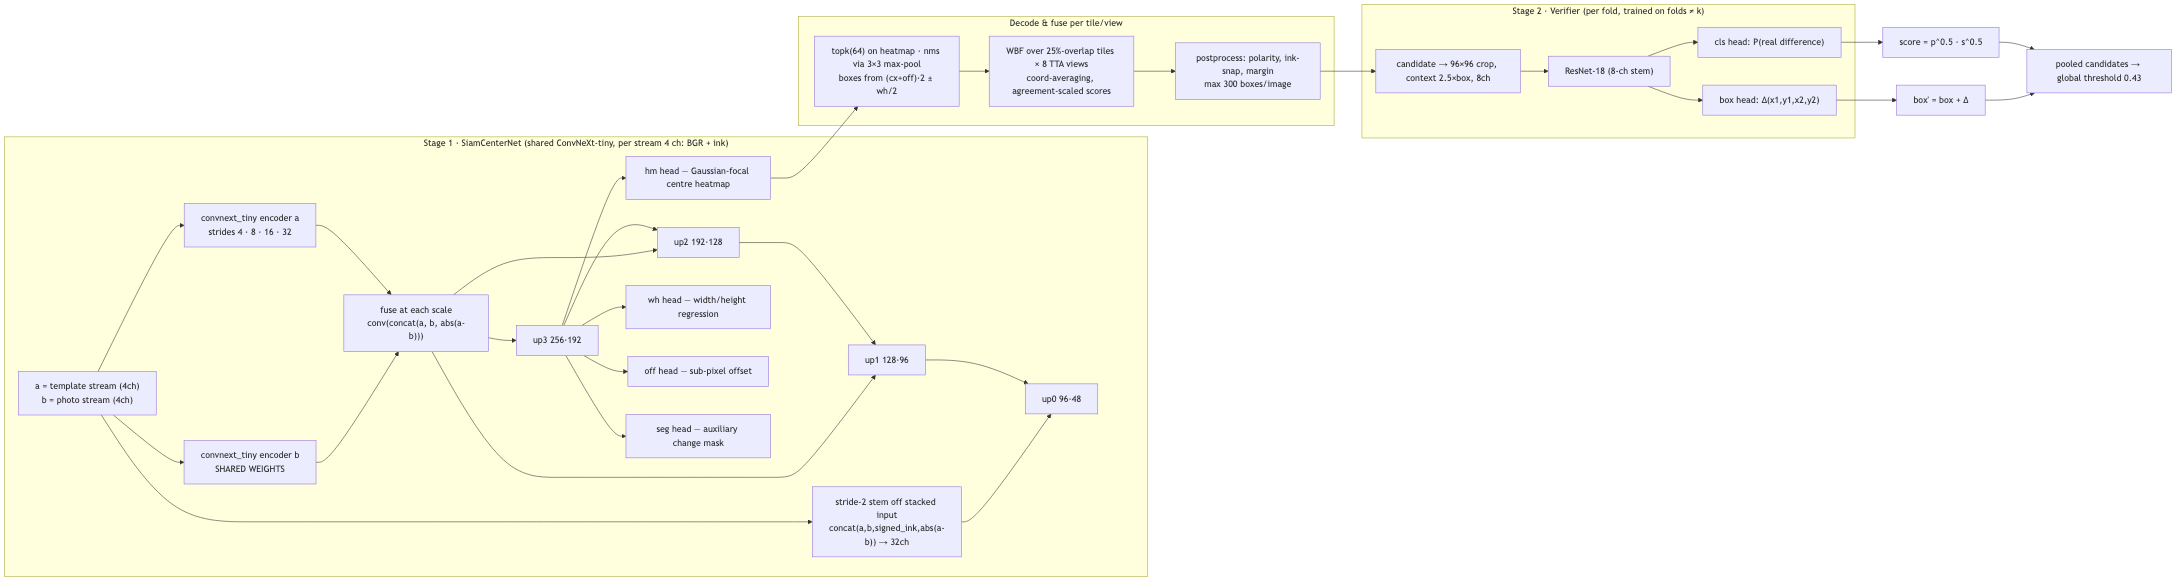
\includegraphics[width=\textwidth]{../diagrams/model_internals.png}
\caption{Model internals --- encoder backbone, fusion blocks and the four detection heads.}
\label{fig:internals}
\end{figure}

\subsection{Stage 2 --- patch verifier (\texttt{src/pmdm/verifier.py})}

96$\times$96 crops around each candidate through a ResNet-18 with an 8-channel stem, producing a
real-difference probability and a box-corner delta. Its probability is blended with the detector
score $p^{0.5}\cdot s^{0.5}$.

\subsection{Stage 3 --- decoding (\texttt{src/pmdm/decode.py})}

Weighted Boxes Fusion (WBF) across overlapping tiles and TTA views (averaging coordinates beats
discarding them when boxes are 8\,px), the polarity filter (0 deletions), ink snapping to the
local difference blob with a measured constant margin, and a single global threshold swept on
out-of-fold predictions.

\section{Cross-validation protocol (the decisive number)}

Five folds over the 200 pairs (seeded split, 40 validation pairs each). For fold $k$:

\begin{enumerate}[leftmargin=1.6em]
\item Two detector recipes (\texttt{\_aug} plain, \texttt{\_augsyn} synthetic) train on the other
160 pairs $+$ \textbf{fold-safe} synthetic pairs (any pair synthesized from a fold-$k$ validation
template is dropped --- 836--892 of 6{,}400 per fold).
\item The 40 held-out pairs are predicted by the ensemble of those two models $+$ 8-view TTA ---
models that never trained on them ($\rightarrow$ \texttt{fold\{k\}\_...\_ens.npz}).
\item The verifier for fold $k$ trains \textbf{only on candidates from folds $\neq k$}, then
rescores fold $k$.
\item All 200 pairs' candidates are pooled and \textbf{one global threshold} (0.43) is swept on
OOF predictions only; F1 is computed globally, exactly as the competition scores a submission.
\end{enumerate}

\begin{figure}[h!]
\centering
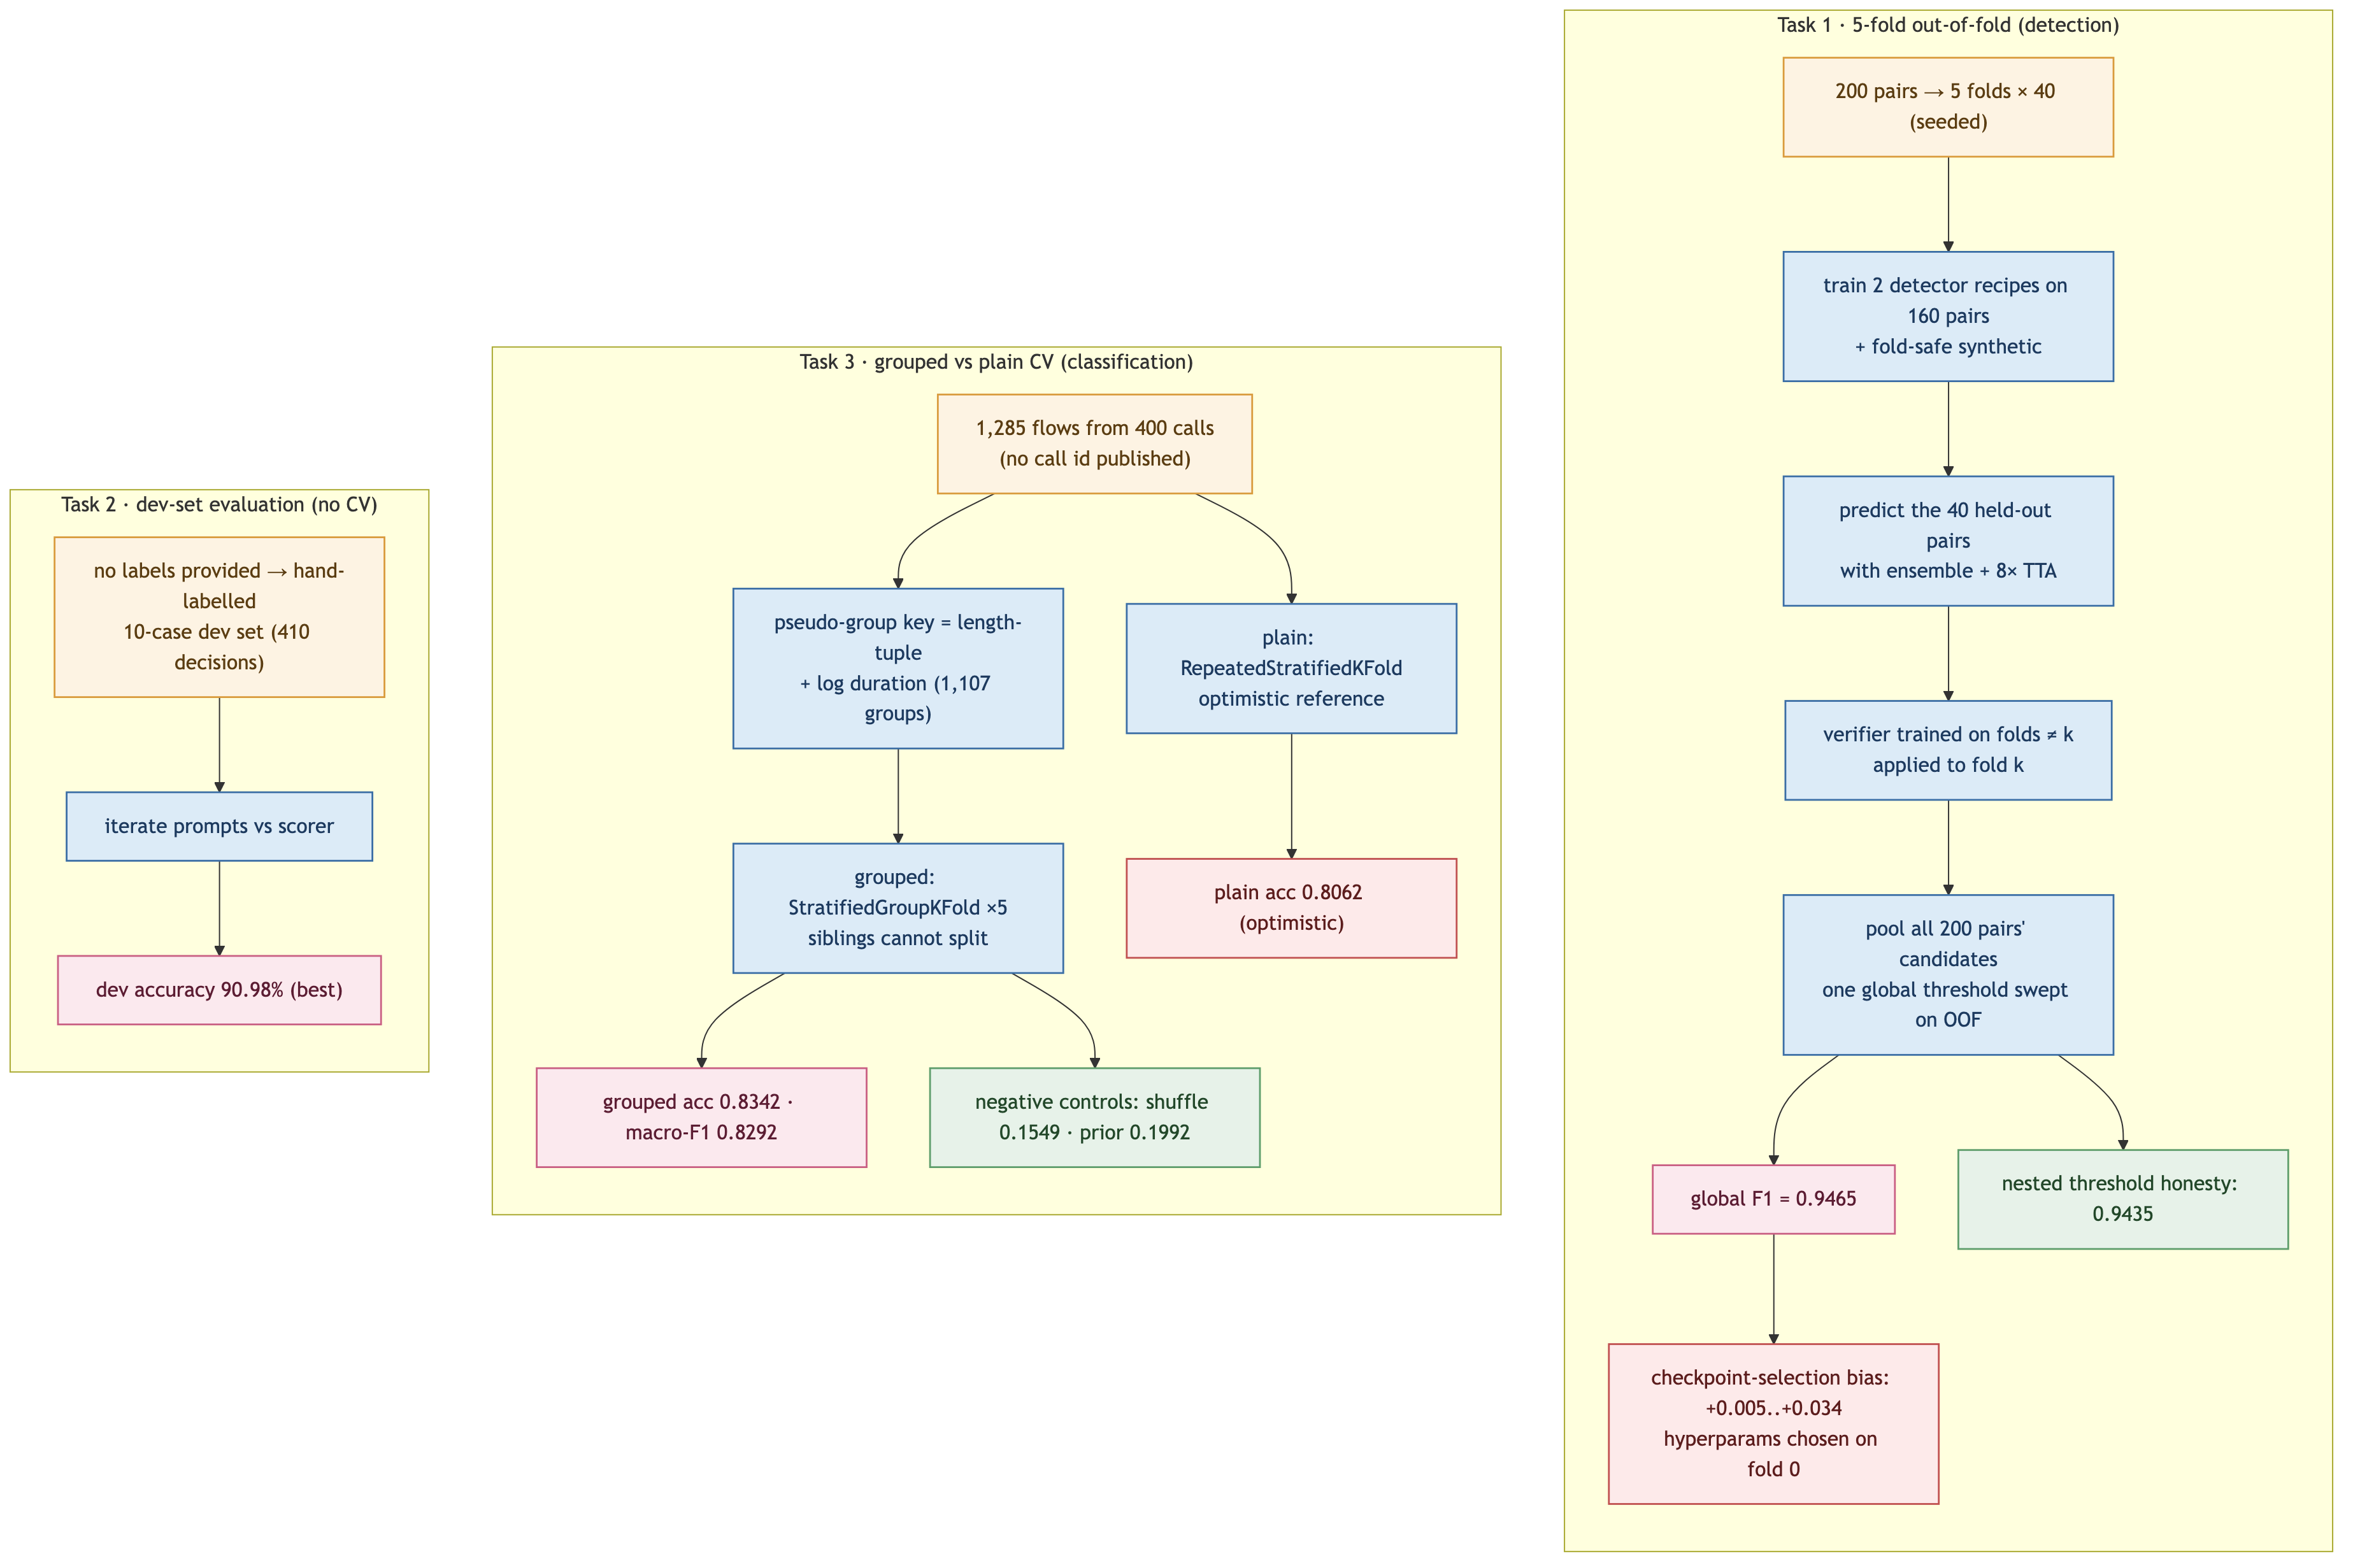
\includegraphics[width=0.9\textwidth]{../report/diagrams/cv_protocol.png}
\caption{Cross-validation protocol: fold-safe synthesis, disjoint detectors, cross-fold verifier,
and pooled global-threshold scoring.}
\label{fig:cv}
\end{figure}

\section{What was tried, and what each thing was worth}

Work proceeded as controlled experiments on fold 0 against a 0.9049 reference; whatever won was
applied to all five folds.

\subsection{Training-side changes}

\begin{table}[h!]
\centering
\small
\renewcommand{\arraystretch}{1.2}
\begin{tabular}{@{}p{4.6cm}p{2.6cm}p{7.8cm}@{}}
\toprule
\textbf{Change} & \textbf{Verdict} & \textbf{Evidence} \\
\midrule
Dihedral augmentation (flips + transpose) & \cmark & \S 5.2 --- worth nothing at old decode settings, $+$0.021 at the right ones \\
Size-relative wh loss & \xmark & fold 0 finished TP 238 / FP 20 / FN 30 --- the reference's counts exactly \\
EMA weights (decay 0.999) & neutral & never selected over raw weights until the last two epochs, where it tied \\
Synthetic small-mark pairs & \cmark~(indirectly) & own F1 worse (0.896 vs 0.926); earns its place through coverage (\S 6) \\
\bottomrule
\end{tabular}
\end{table}

\textbf{Lesson from the first three rows:} on 268 validation boxes, one box is worth 0.004 F1 and
the run-to-run spread is $\pm$0.02. Three independent runs landed between 0.890 and 0.905.
Nothing inside that band is a result.

\subsection{The decode settings mattered more than the training changes}

The augmented model scored 0.9049 at the reference decode settings (\texttt{score\_thr 0.05},
\texttt{max\_boxes 40}, no TTA) and \textbf{0.9257} at \texttt{score\_thr 0.02},
\texttt{max\_boxes 300}, 8-view TTA --- the same weights, $+$0.021. Every earlier comparison had
been made through a lossy decoder, which is why augmentation looked worthless. Model quality and
decode quality are not separable; comparing models at their default decode is comparing decoders.

\begin{table}[h!]
\centering
\small
\renewcommand{\arraystretch}{1.2}
\begin{tabular}{@{}p{8.2cm}c@{}}
\toprule
\textbf{Setting} & \textbf{fold-0 F1} \\
\midrule
reference (\texttt{score\_thr 0.05}, cap 40, no TTA) & 0.9049 \\
\texttt{score\_thr 0.02}, cap 300, 8-view TTA & \textbf{0.9257} (same weights, $+$0.021) \\
\bottomrule
\end{tabular}
\end{table}

\subsection{The verifier --- positive on all five folds}

Retrained on generous candidate sets ($\sim$11{,}000 records per fold at an 8:1
negative:positive ratio), trained per fold on the four folds it would never be applied to:

\begin{table}[h!]
\centering
\small
\renewcommand{\arraystretch}{1.2}
\begin{tabular}{@{}cccr@{}}
\toprule
\textbf{fold} & \textbf{before} & \textbf{after} & $\Delta$ \\
\midrule
0 & 0.9266 & 0.9430 & $+$0.016 \\
1 & 0.9414 & 0.9551 & $+$0.014 \\
2 & 0.9288 & 0.9347 & $+$0.006 \\
3 & 0.9544 & 0.9609 & $+$0.006 \\
4 & 0.9494 & 0.9676 & $+$0.018 \\
\bottomrule
\end{tabular}
\end{table}

\section{Recall ceilings --- the measurement that redirected everything}

The ceiling is the fraction of ground-truth boxes present \emph{anywhere} in the candidate list at
IoU 0.5, regardless of score. Nothing downstream can recover a box that was never proposed, so
this bounds every rescoring idea.

\begin{table}[h!]
\centering
\small
\renewcommand{\arraystretch}{1.2}
\begin{tabular}{@{}p{5.0cm}ccccc@{}}
\toprule
\textbf{Model (fold 0, TTA, score 0.02)} & \textbf{candidates} & \textbf{ceiling} & \textbf{$<$12\,px ceiling} & \textbf{best F1} \\
\midrule
original single model & 421 & 0.9403 & 0.828 & 0.9049 \\
\texttt{\_aug} & 2{,}770 & 0.9440 & 0.891 & 0.9257 \\
\texttt{\_augpix} & 3{,}602 & 0.9478 & 0.844 & 0.9185 \\
\texttt{\_augsyn} (synthetic) & 10{,}238 & 0.9590 & \textbf{0.922} & 0.8956 \\
\textbf{\texttt{\_aug} $+$ \texttt{\_augsyn}} & 10{,}389 & \textbf{0.9627} & \textbf{0.9375} & \textbf{0.9266} \\
\texttt{\_aug} $+$ \texttt{\_augpix} $+$ \texttt{\_augsyn} & 10{,}826 & 0.9590 & 0.9375 & 0.9251 \\
\bottomrule
\end{tabular}
\end{table}

This is where the synthetic data justified itself. Sub-12\,px coverage went from 0.828 to 0.922 ---
and that band previously held 10 of the 11 boxes the model missed entirely. The synthetic model's
own F1 is poor because it proposes aggressively; that is a \emph{scoring} problem, and scoring is
fixable. Three models were worse than two: \texttt{\_augpix} adds candidates without adding
coverage, so it only dilutes the agreement signal.

\section{Final results}

\textbf{Pooled over all 200 pairs and all 1{,}407 boxes, one global threshold, each pair predicted
only by models that never trained on it:}

\begin{table}[h!]
\centering
\small
\renewcommand{\arraystretch}{1.25}
\begin{tabular}{@{}lcccccc@{}}
\toprule
\textbf{Stage} & \textbf{F1} & \textbf{Precision} & \textbf{Recall} & \textbf{TP} & \textbf{FP} & \textbf{FN} \\
\midrule
Classical baseline & 0.0293 & 0.015 & 0.572 & --- & --- & --- \\
Original single model (fold 0) & 0.9049 & 0.922 & 0.888 & 238 & 20 & 30 \\
Ensemble + TTA & 0.9385 & 0.962 & 0.916 & 1{,}289 & 51 & 118 \\
\textbf{$+$ verifier} & \textbf{0.9465} & \textbf{0.963} & \textbf{0.930} & \textbf{1{,}309} & \textbf{50} & \textbf{98} \\
$+$ verifier, nested threshold (\S 8) & 0.9435 & --- & --- & --- & --- & --- \\
\bottomrule
\end{tabular}
\end{table}

Per-fold, ensemble $+$ verifier: \textbf{0.943, 0.955, 0.935, 0.961, 0.968}. Fold 0 --- the fold
every early experiment was measured on --- is the hardest of the five.

\textbf{Submission:} 668 boxes over 100 test images (6.68 per image against a training average of
7.04). Produced by all ten detectors ensembled with TTA, all five verifiers averaged, threshold
0.43.

\section{Leakage discipline}

Four rules, each enforced in code rather than by convention:

\begin{enumerate}[leftmargin=1.6em]
\item \textbf{Synthetic pairs are fold-scoped.} A synthetic pair carries invented boxes but the
\emph{real page layout} it was built from. Every pair records its source template, and each fold
discards any pair derived from its own validation pages (836--892 of 6{,}400 pairs per fold).
\item \textbf{Test templates are a legitimate synthesis source.} They carry no labels, so nothing
can leak; they contribute 100 layouts no model would otherwise see.
\item \textbf{The verifier for fold $k$ trains only on candidates from folds $\neq k$}, themselves
produced by detectors that never saw those pages.
\item \textbf{One global threshold, swept on out-of-fold predictions only} --- never on the fold
being reported, never on test.
\end{enumerate}

Out-of-fold scoring uses one model pair per image; the test submission uses all ten. The test score
should therefore land slightly \emph{above} the reported out-of-fold figure.

\section{Is it overfit?}

Three places where selection touched the reported number.

\textbf{Threshold selection --- measured, negligible.} Nested cross-validation, choosing the
threshold on four folds and applying it to the fifth:

\begin{table}[h!]
\centering
\small
\renewcommand{\arraystretch}{1.25}
\begin{tabular}{@{}lccc@{}}
\toprule
 & \textbf{tuned on eval} & \textbf{nested honest} & \textbf{optimism} \\
\midrule
detector only & 0.9385 & 0.9385 & $+$0.0000 \\
$+$ verifier & 0.9465 & 0.9435 & $+$0.0030 \\
\bottomrule
\end{tabular}
\end{table}

\textbf{Checkpoint selection --- the real bias.} \texttt{train\_fold} evaluates on the fold's own
validation pairs and saves \texttt{best.pt} at the highest-scoring epoch; reporting that
checkpoint on those same pairs is taking the max of eight noisy measurements:

\begin{table}[h!]
\centering
\small
\renewcommand{\arraystretch}{1.25}
\begin{tabular}{@{}lcc@{}}
\toprule
\textbf{recipe} & \textbf{mean} & \textbf{range} \\
\midrule
\texttt{\_aug} & $+$0.005 & 0.000 -- 0.011 \\
\texttt{\_augsyn} & \textbf{$+$0.034} & 0.020 -- 0.058 \\
\bottomrule
\end{tabular}
\end{table}

The \texttt{\_aug} curves are flat at the end; the \texttt{\_augsyn} models trained only 15 epochs
and were still oscillating, so \texttt{best.pt} cherry-picks a lucky point.

\textbf{Hyperparameter selection.} \texttt{score\_thr}, \texttt{max\_boxes}, the TTA configuration
and the two-model ensemble pairing were all chosen on fold 0, then applied to all five ---
contaminating one fifth of the pooled number. Unquantified; probably small, certainly not zero.

\textbf{Honest estimate of true generalization: 0.925--0.94} (not 0.9465). Counter-evidence
against serious overfitting: the test set yields 6.68 boxes per image against out-of-fold's 6.80
and ground truth's 7.04 --- no distribution shift on unseen data --- and the verifier improved all
five disjoint folds independently.

\section{What is left, and what is reachable}

The candidate set contains 1{,}352 of 1{,}407 boxes at IoU 0.5 --- a \textbf{ceiling of 0.9609}.
A rescorer that never erred would therefore score:

\begin{center}
TP 1{,}352,\; FP 0,\; FN 55 \quad$\Rightarrow$\quad P 1.000,\; R 0.961,\; \textbf{F1 0.9801}
\end{center}

The 0.97 target sits above what perfect rescoring of the current proposals can deliver, and the
pipeline is already within 0.014 of that unreachable bound. The 98 false negatives split into 55
boxes no model proposes at all and 43 proposed but below threshold; there are 50 false positives.

The 55 are the frontier --- reaching them means better \emph{proposals}, not better scoring. The
sub-12\,px band that used to dominate misses is now at 0.944 coverage, so that lever is largely
spent. Plausible next moves, in order worth trying:

\begin{enumerate}[leftmargin=1.6em]
\item \textbf{Remove checkpoint-selection bias} (\S 8) so future comparisons are trustworthy.
\item \textbf{Train \texttt{\_augsyn} properly} --- 15 epochs left it undertrained (final epoch
0.81 vs best 0.87); a 40-epoch run should raise both its own F1 and the ensemble's ceiling.
\item \textbf{Inspect the 55 missed boxes directly} --- whatever they have in common is the next
architectural change.
\item \textbf{A second backbone} (ConvNeXt-small, or a different family) for genuine ensemble
diversity --- \texttt{\_augpix} failed because it was too similar to \texttt{\_aug}.
\end{enumerate}

\section{Bugs found}

All four were silent --- they produced wrong numbers rather than errors.

\begin{enumerate}[leftmargin=1.6em]
\item \textbf{WBF score saturation.} The fused confidence divided by a cap of 3, so any box agreed
on by more than three views saturated at 1.0 while a box proposed by a single view kept its full
raw score --- confidence effectively inverted. A TTA run scored 0.775 at precision 0.67 because of
it, which read as ``TTA doesn't work''. Fixed to the standard agreement-scaled mean.
\item \textbf{Ensemble double-counted its sources.} Members already fuse their own views, so
pooling with $n_{\mathrm{sources}} = \mathrm{models}\times\mathrm{views}$ divided every score by
$\sim$16; recall collapsed to 0.056.
\item \textbf{Verifier data loading.} It re-decoded four full-page PNGs per sample on every cache
miss and shuffled across 160 pages ($\sim$140{,}000 decodes, $\sim$60 min/epoch with the GPU
idle). Crops are now cut once into memory: seconds per epoch.
\item \textbf{\texttt{--detach} does not protect \texttt{starmap}.} The fan-out is client-driven,
so a network blip killed an entire five-way map. Fan-out now happens inside a remote function.
\end{enumerate}

\section{Artifacts and reproduction}

\begin{table}[h!]
\centering
\small
\renewcommand{\arraystretch}{1.2}
\begin{tabular}{@{}p{4.6cm}p{10.4cm}@{}}
\toprule
\textbf{Path} & \textbf{Contents} \\
\midrule
\texttt{submission.csv} & 668 boxes, 100 images, format-validated against \texttt{train.csv} \\
\texttt{RESULTS.md} & condensed results summary \\
\texttt{PLAN\_097.md} & the plan as written \emph{before} the work, kept for comparison \\
\texttt{checkpoints/} & all 16 models: 10 detectors, 5 verifiers, plus the original \\
\texttt{runs/phase2/} & per-fold candidates before/after verification, filtered logs \\
\texttt{src/pmdm/} & 16 modules \\
\texttt{RUNBOOK.md} & the exact command sequence that produced these numbers \\
\bottomrule
\end{tabular}
\end{table}

Full pipeline, roughly 2 hours wall clock: synthetic corpus (16 CPU shards) $\rightarrow$ 10
detectors (8$\times$A100, $\sim$1\,h) $\rightarrow$ ensemble out-of-fold candidates (5$\times$L4)
$\rightarrow$ verifiers (5$\times$L4) $\rightarrow$ pooled score $\rightarrow$ submission
(5$\times$L4). Estimated total compute spend: \textbf{\$35--40}, dominated by A100 fold training.

\section{Summary of the through-line}

The single most useful thing done in this project was not an architectural change: it was measuring
the \textbf{recall ceiling} separately from F1. That number showed the synthetic-data model ---
which looked like a clear failure at 0.896 F1 --- held the best candidate coverage by a wide
margin, and that the whole rescoring branch was bounded at 0.98 no matter how good the verifier
became. Both facts redirected the work, and neither was visible in the headline metric.

The second most useful was distrusting flat comparisons: three ``no gain'' verdicts on augmentation
were artefacts of comparing models through a lossy decoder, and one ``TTA is worse'' verdict was a
scoring bug. Every one of those was reported as a negative result before being found to be wrong.

\end{document}
